\documentclass{article}
\usepackage{polski}
\usepackage{graphicx} 
\usepackage[utf8]{inputenc}
\title{Opis modelów sieciowych TCP/IP i ISO/OSI}
\date{\today}
\author{Jakub Kołomański}
 \begin{document}
   \maketitle
  \begin{thebibliography}{9}
  \bibitem{Model TCP/IP}
  Wikipedia.org
  \textit{Model TCP/IP},
  Społeczeństwo Wikipedia,
  
  \end{thebibliography}
  \newpage
 \section{Model TCP/IP}
\subsection{Opis}
	Model TCP/IP (ang. Transmission Control Protocol/Internet Protocol) – teoretyczny model warstwowej struktury protokołów komunikacyjnych. Model TCP/IP został stworzony w latach 70. XX wieku w DARPA, aby pomóc w tworzeniu odpornych na atak sieci komputerowych. Potem stał się podstawą struktury Internetu.
	
Podstawowym założeniem modelu TCP/IP jest podział całego zagadnienia komunikacji sieciowej na szereg współpracujących ze sobą warstw (ang. layers). Każda z nich może być tworzona przez programistów zupełnie niezależnie, jeżeli narzucimy pewne protokoły według których wymieniają się one informacjami. Założenia modelu TCP/IP są pod względem organizacji warstw zbliżone do modelu OSI. Jednak liczba warstw jest mniejsza i bardziej odzwierciedla prawdziwą strukturę Internetu. Model TCP/IP składa się z czterech warstw.

Każdy protokół sieciowy można przyporządkować do określonej warstwy modelu TCP/IP. Pewną szczególną cechą rodziny protokołów TCP/IP używanej w Internecie jest podział protokołów z warstwy aplikacyjnej i połączeniowej. Niektóre protokoły z warstwy aplikacji wykorzystują tylko pewne protokoły z warstwy transportowej.

Protokoły DNS, NTP wykorzystują tylko protokół UDP z warstwy transportowej. Protokoły FTP, SMTP, POP3, SSH, IRC posługują się tylko TCP. Natomiast SMB używa obu protokołów.

Protokół SSL ma szczególną rolę. Może zostać umieszczony pomiędzy każdym połączeniowym protokołem warstwy aplikacji a TCP. Dzięki jego wykorzystaniu dane przesyłane przez aplikacje mogą zostać zaszyfrowane.

Niektóre protokoły z warstwy aplikacji, jak np. SMB nie działają zwykle w Internecie. Są wykorzystane w sieciach lokalnych do udostępniania usług, jak np. zdalne drukarki czy dyski.

W systemie GNU/Linux oraz innych odpowiednikach Uniksa dokładną listę protokołów transportowych można znaleźć w pliku.

W dzisiejszych czasach, praktycznie każdy system operacyjny posiada domyślnie zainstalowane protokoły TCP/IP.

Istnieje także Lightweight TCP/IP, szerzej znany jako darmowy stos TCP/IP dla systemów wbudowanych, czyli będących integralną częścią obsługiwanego przez nie sprzętu - jest to stos protokołów dla systemów obsługujących zarówno amatorskie jak i zaawansowane urządzenia, często budowane z wykorzystaniem programowalnych układów FPGA (np. sprzętowe serwery WWW, FTP). Istnieją także proste stosy TCP/IP realizowane całkowicie sprzętowo.
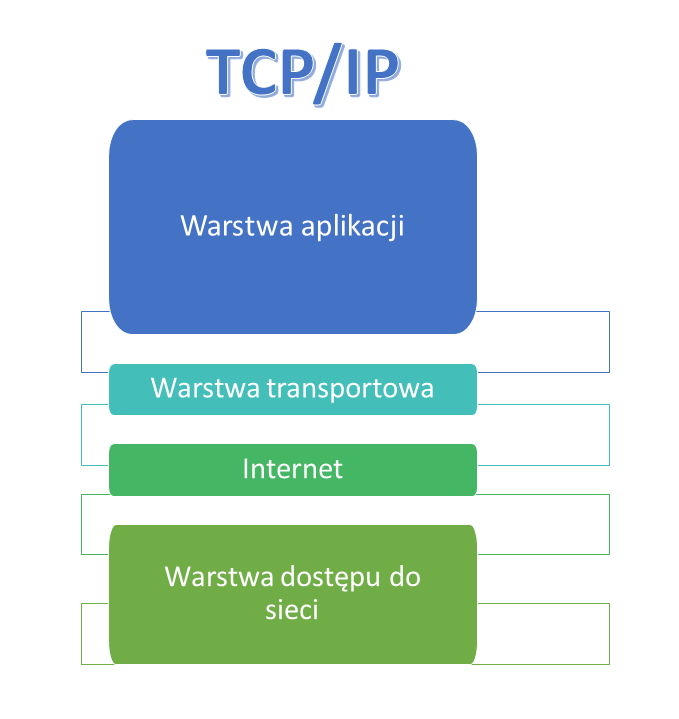
\includegraphics[width=0.7\textwidth]{tcp.png}

\section{Model ISO/OSI}
\subsection{Opis}
	Model OSI (pełna nazwa ISO OSI RM, ang. ISO Open Systems Interconnection Reference Model – model odniesienia łączenia systemów otwartych) lub OSI – standard zdefiniowany przez ISO oraz ITU-T opisujący strukturę komunikacji sieciowej.

Międzynarodowa Organizacja Normalizacyjna (ang. International Organization for Standardization) na początku lat osiemdziesiątych dostrzegła potrzebę stworzenia modelu sieciowego, dzięki któremu producenci mogliby opracowywać współpracujące ze sobą rozwiązania sieciowe. W taki sposób powstała specyfikacja Open Systems Interconnection Reference Model, która do polskich norm została zaadaptowana w 1995 roku.

Model ISO OSI RM jest traktowany jako model odniesienia (wzorzec) dla większości rodzin protokołów komunikacyjnych. Podstawowym założeniem modelu jest podział systemów sieciowych na 7 warstw (ang. layers) współpracujących ze sobą w ściśle określony sposób. Został przyjęty przez ISO w 1984 roku a najbardziej interesującym organem jest wspólny komitet powołany przez ISO/IEC, zwany Joint Technical Committee 1- Information Technology (JTC1). Formalnie dzieli się jeszcze na podkomitety SC.
 
 Model OSI definiuje jakie zadania oraz rodzaje danych mogą być przesyłane między warstwami w całkowitym oderwaniu od ich fizycznej i algorytmicznej realizacji, czyli zakłada istnienie warstw abstrakcji w medium transmisyjnym, sprzęcie oraz oprogramowaniu i wokół tych warstw orientuje specyficzne dla nich protokoły, realizowane przez te protokoły usługi świadczone wyższym warstwom oraz posiadane interfejsy, umożliwiające dostęp do warstwy przez procesy z innych warstw. Mimo iż każda z warstw sama nie jest funkcjonalna, to możliwe jest projektowanie warstwy w całkowitym oderwaniu od pozostałych. Jest to realne, jeżeli wcześniej zdefiniuje się protokoły wymiany danych pomiędzy poszczególnymi warstwami.
 
 W praktyce Model OSI został częściowo zmodyfikowany. Najczęstszą zmianą było połączenie warstwy fizycznej oraz łącza danych w jedną. Wynikało to z praktycznych cech tych warstw, które powodowały, że nie dało się odseparować ich pracy od siebie. Nie należy mylić Modelu OSI-RM z TCP/IP. Mimo pewnego podobieństwa oba te modele nie są w pełni zgodne.
 


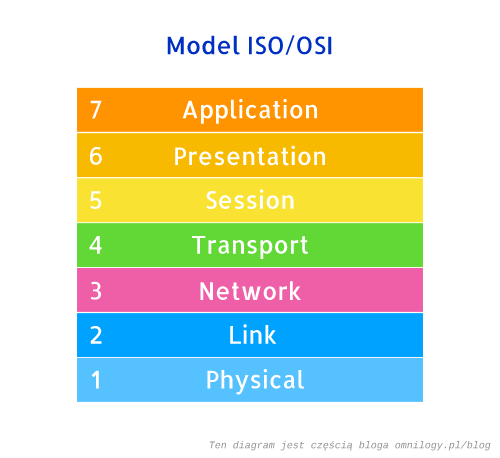
\includegraphics[width=0.6\textwidth]{OSI.png}

 \end{document}